\subsubsection{Acoustic Complexity Index}
\par The emerging field of soundscape ecology focuses on using the sounds in an environment to analyze, predict and correct the problems within that environment. These problems are often caused by the ever-present human expansion into previously undisturbed natural habitats. This invasion of habitats means that the organisms that live there are constantly forced leave due to the increase in human made machine noise (Anthrophony). This Anthrophony disrupts the organism's natural communication, since most organisms rely on sound to communicate. Those organisms that choose to stay and overcome the noise leave a sonic footprint within the environment itself. Often this footprint can tell a story about the troubles with biodiversity in an area. This is where the Acoustic Complexity Index or ACI comes into play. First used in Tuscan Emilian Apennine National Park, Italy; The ACI measures the change in acoustic intensity. This allows for researchers to pinpoint areas of interesting sound within a recording, even through human made machine noise or Anthrophony. Allowing for research of the biodiversity in areas that have been tainted with human sound.
\begin{center}
  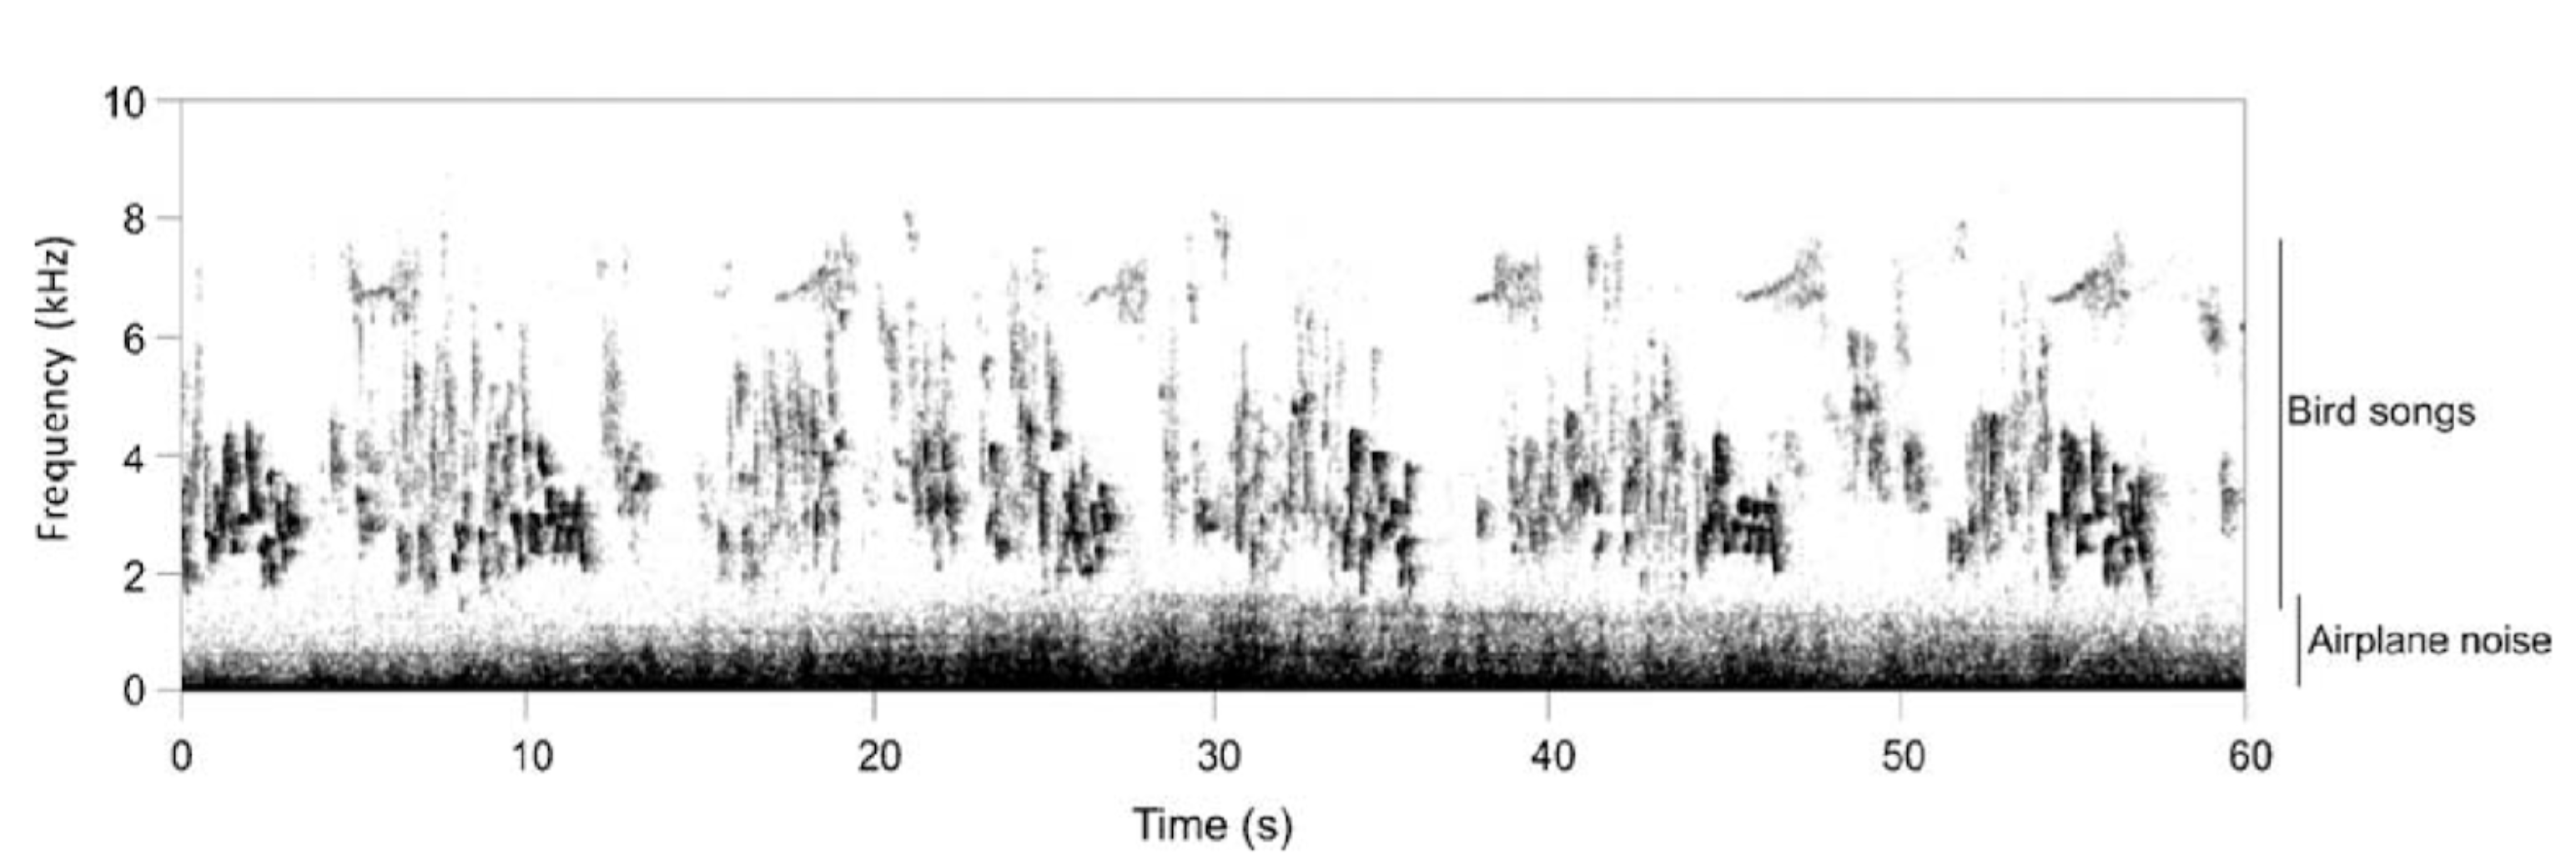
\includegraphics[width=0.85\textwidth]{ACI} \\[12pt]
\end{center}
\par ACI relies on the fact that most Biophonic (non-human biological sounds) have a high level of complexity when it comes to their intensity. Meaning that most natural sounds have a high variance of loudness. This is in stark contrast with the mostly monotone nature of human made sounds. This key difference in sound types allows the ACI to filter out plane noises or car sounds amongst bird sounds and other Biophonic interests. When compared to the previous technique of cutting off at certain sound frequency indexes, the ACI tends to save useful data from being truncated and lost.
\par During a trial done by N. Pieretti the ACI was shown to have a high correlation with the number of bird vocalizations in an area. This comparison was done by placing 20 digital recorders 100m apart in a 4x5 grid in the previously mentioned Italian park. Areas that were recorded to have high levels of bird sound also had a correlated high ACI.
\begin{quote}
 ``The strong correlation between the ACI and the singing activity of the avian community
  is related to the capacity of this index to successfully highlight rapid variations of the
  intensity in each single frequency bin, a feature that is typical of bird songs.''\cite{pieretti}
\end{quote}

Increasing the length of sound track that was analyzed also increased in a correlation between ACI and number of bird vocalizations.

\begin{center}
  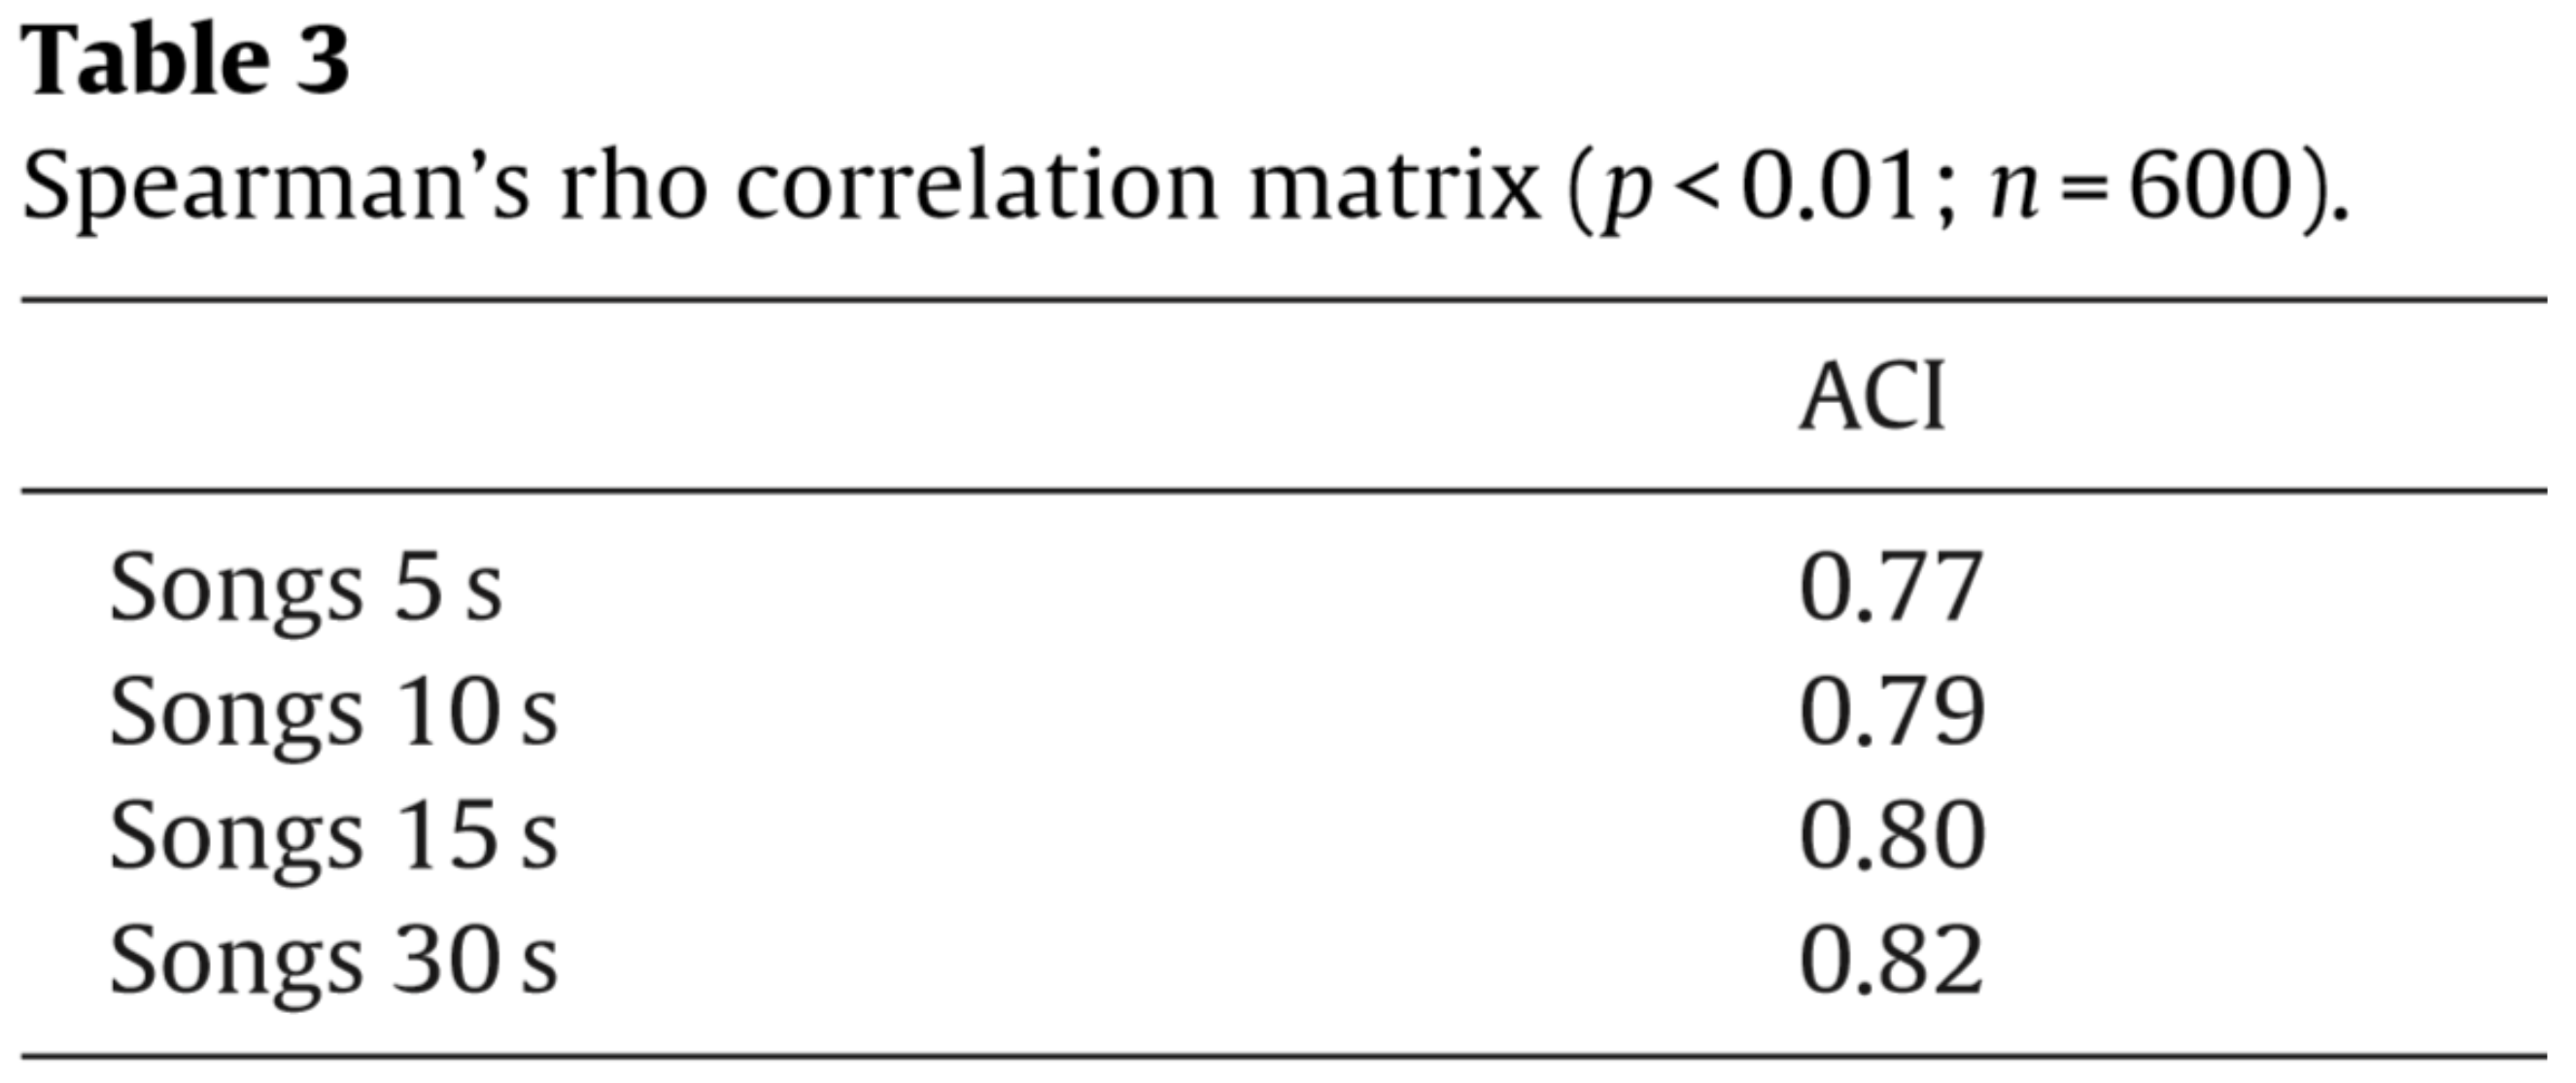
\includegraphics[width=0.85\textwidth]{RhoCorrelation} \\[12pt]
\end{center}

\par While there is a promising amount of research for the ability of the ACI to discriminate between Anthrophony and Biophony, the algorithm still does very poorly in discerning between different types of Biophony and Geophony. This challenge can be highlighted by the fact that the algorithm produces high numbers for sounds such as buzzing insects and wind. Both of which have high variance of intensity and thus increase the ACI value for a given sound bucket. Along this same strain of problem, the ACI cannot differentiate between species or even types of animal sounds. This type of classification is still left up to techniques such as model recognizers; models that are built to recognize one type of species. In the study, the Wildlife Acoustics program was used to build these recognition models and provide a benchmark for the accuracy of the ACI.
\par The ACI, in combination with other measuring techniques, can be a powerful tool for finding the Biophonic sounds within a recording. These types of breakthroughs in soundscape ecology allow professional Ornithologists to conduct research efficiently without ever having to travel into the field. Hopefully our Senior Design project will allow researchers and other interested individuals to access these algorithms and use them to analyze the effects of human made sounds on the surrounding habitats.\cite{pieretti}
